%!TEX program = xelatex
\documentclass[xcolor={table}]{beamer}

\usepackage[brazil]{babel}	
\usepackage[utf8]{inputenc}
\usepackage[T1]{fontenc}
\usepackage[scaled]{helvet}
\usepackage{amsthm}
\usepackage{ragged2e}
\usepackage{subfig}
\usepackage[table]{xcolor}
\usepackage{multicol}
\usepackage{multirow}
\usepackage{fancyvrb}
\usepackage{verbatim}
\usepackage{hyperref}

\usetheme{Execushares}

\title{Laborator 0 - Introducere}
\subtitle{}
\author{
        Coca Mihai\\
        Ioana Dragoș
        }

\setcounter{showSlideNumbers}{1}

\begin{document}
	\setcounter{showProgressBar}{0}
	\setcounter{showSlideNumbers}{0}

	\frame{\titlepage}

	\begin{frame}
		\frametitle{Tabelă de Conținut}
		\begin{enumerate}
			\item Noțiuni administrative
			\item Instrumente
			\item Mediul de lucru
			\item Utile
		\end{enumerate}
	\end{frame}

	\setcounter{framenumber}{0}
	\setcounter{showProgressBar}{1}
	\setcounter{showSlideNumbers}{1}
	\section{Noțiuni administrative}
		\begin{frame}
			\frametitle{Administrativ}
			\begin{itemize}
			    \item \textbf{Resurse}: \href{https://wiki.mta.ro/c/4/ssmp/start}{Wiki}
			    \item \textbf{Suport Laborator}: \href{https://github.com/undacmic/MCULabs}{MCULabs}
			    \item \textbf{Echipa}: \textit{Mihai COCA}, \textit{Dragoș IOANA}
			    \item Componența grupei în format XLSX
			    
			\end{itemize}
		\end{frame}

		\begin{frame}
			\frametitle{Notare}
			\begin{enumerate}
				\item Notă finală
					\begin{itemize}
    			        \item Curs ($ 60\% $ din notă)
    			        \item Laborator ($ 40\% $ din notă)
    			    \end{itemize}
				\item \textbf{Atenție: Este necesară promovarea independentă curs + laborator!}
			\end{enumerate}
		\end{frame}
		
		\begin{frame}
			\frametitle{Proiect}
			\begin{enumerate}
			    \item Echipă
			    	\begin{itemize}
    			        \item Formată din 3 studenți, cu posibilitatea de vizualizare în cadrul unui XLSX
    			        \item Va avea desemnat un responsabil pentru resursele primite
    			    \end{itemize}
				\item Componență
					\begin{itemize}
    			        \item Document ce conține specificația proiectului: scop, resurse folosite, module configurate, detalii rulare, probleme întâmpinate,  soluționări și îmbunătățiri, concluzii
    			        \item Cod sursă
    			    \end{itemize}
				\item Evaluare
					\begin{itemize}
    			        \item Evaluare periodică - actualizare asupră stării proiectului + feedback
    			        \item Evaluare finală (ultimele 2 module)
    			    \end{itemize}
			\end{enumerate}
		\end{frame}

	\section{Instrumente}
    	\begin{frame}
    		\frametitle{\textit{Must-have}}
    		\begin{itemize}
    		    \item Resurse
    		        \begin{itemize}
        				\item \href{https://www.keil.com/download/product/}{\textbf{ARM Keil} - \textit{MDK-Arm} Pack}
        				\item \href{https://studio.keil.arm.com/}{\textbf{Keil Studio Cloud}}
    		        \end{itemize}
    		\end{itemize}
    	\end{frame}

    	\begin{frame}
    		\frametitle{\textit{Nice to Have}}
    		\begin{itemize}
    			\item Cunoștințe despre dispozitive și circuite electronice
    			\item Experiență cu C
    		\end{itemize}
    	\end{frame}

	\section{Mediul de lucru}
		\begin{frame}
			\frametitle{Platformă}
			\begin{itemize}
				\item \textbf{FRDM-KL25Z} - ARM® Cortex™-M0+ Core, 48MHz, 16KB RAM, 128KB FLASH
			\end{itemize}
			\begin{figure}
                \centering
                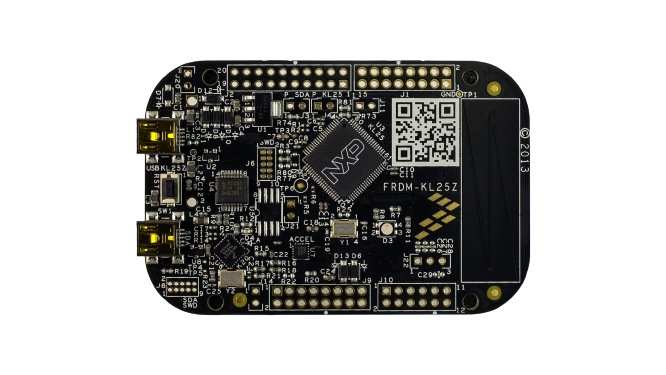
\includegraphics[width=9cm]{images/FRDM-KL25Z.png}
            \end{figure}
		\end{frame}
		
		\begin{frame}
			\frametitle{Componente periferice}
			\begin{enumerate}[<+->]
				\item \textbf{UART} - comunicație serială asincronă
				\item \textbf{SPI, I2C} - comunicație serială sincronă
				\item \textbf{GPIO} - Input/Output
				\item \textbf{PIT} - timer
				\item \textbf{PWM} - power management
				\item \textbf{DAC} - conversie digital în analogic
				\item \textbf{ADC} - conversie analogic în digital
			\end{enumerate}
		\end{frame}
		
		\begin{frame}
			\frametitle{Componente electrice}
			\begin{enumerate}
				\item \textbf{Senzori}
					\begin{itemize}
				        \item \textit{Analogici} (analog input) - 
				        \textbf{Vibrație},
				        \textbf{Sunet}, 
				        \textbf{Rotație}, 
				        \textbf{Flacără}, 
				        \textbf{Lumină Ambientală}
				        \textbf{Gaz}s
				        \item \textit{Digitali}-
				        \textbf{Buzzer} (analog output),
				        \textbf{Temperatură și umiditate} (analog input),
				        \textbf{Vibrație}, 
				        \textbf{Push} (digital input),
				        \textbf{LED},
				        \textbf{BCD} 
			        \end{itemize}
			    \item \textbf{Actuatori} - Motor Servo
				\item \textbf{Breadboard}
				\item \textbf{Rezistori}
			\end{enumerate}
		\end{frame}
		
		\begin{frame}
    		\frametitle{Aplicații}
    			\begin{itemize}
        			\item \href{https://www.hackster.io/projects/tags/microcontroller}{\textbf{Hackster}}
        			\item \href{https://community.nxp.com/}{\textbf{NXP Community}}
        			\item \href{https://os.mbed.com/platforms/KL25Z/}{\textbf{Mbed OS}}
    		    \end{itemize}
    	\end{frame}
	
	\section{Utile}
		
	\begin{frame}
		\frametitle{Documente}
			\begin{itemize}
    			\item \href{https://github.com/undacmic/MCULabs/blob/main/Resurse/FRDM-KL25Z_ReferenceManual.pdf}{\textbf{Reference Manual}}
    			\item \href{https://github.com/undacmic/MCULabs/blob/main/Resurse/FRDM-KL25Z_Schematics.pdf}{\textbf{Schematics}}
    			\item \href{https://github.com/undacmic/MCULabs/blob/main/Resurse/FRDM-KL25Z_UserManual.pdf}{\textbf{User's Manual}}
    			\item \href{https://github.com/undacmic/MCULabs/blob/main/Resurse/FRDM-KL25Z_Datasheet.pdf}{\textbf{Datasheet}}
    			\item \href{https://github.com/undacmic/MCULabs/blob/main/Resurse/FRDM-KL25Z_Pinouts.pdf}{\textbf{Pinouts}}
    			\item \href{https://github.com/undacmic/MCULabs/blob/main/Resurse/KINETIS_L_Errata.pdf}{\textbf{Errata sheet}}
		    \end{itemize}
	\end{frame}


\end{document}